% Created by tikzDevice version 0.12.3.1 on 2022-09-05 08:11:42
% !TEX encoding = UTF-8 Unicode
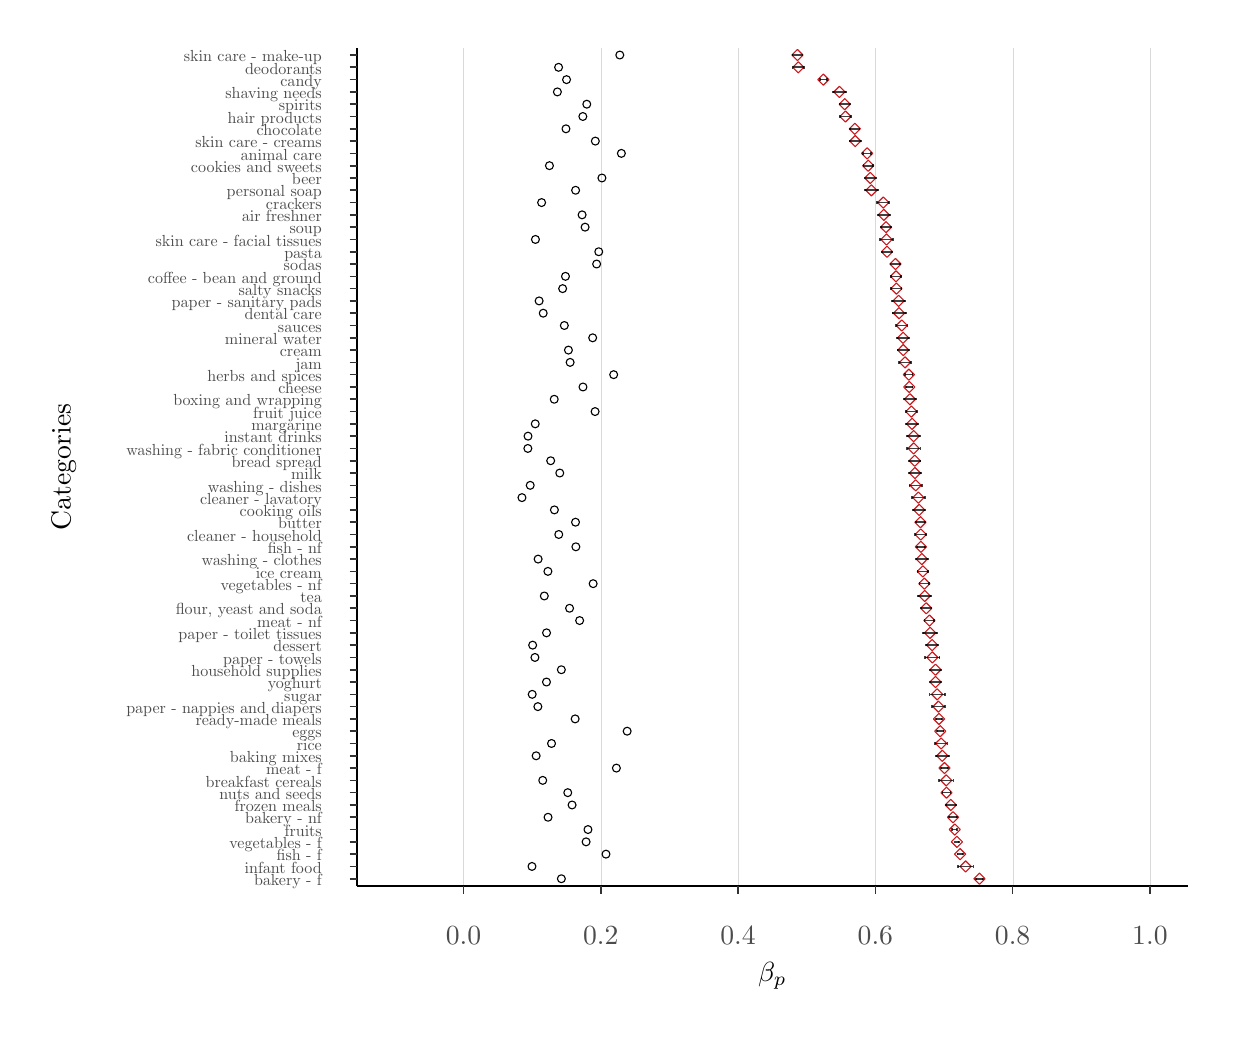
\begin{tikzpicture}[x=1pt,y=1pt]
\definecolor{fillColor}{RGB}{255,255,255}
\path[use as bounding box,fill=fillColor,fill opacity=0.00] (0,0) rectangle (433.62,361.35);
\begin{scope}
\path[clip] (  0.00,  0.00) rectangle (433.62,361.35);
\definecolor{drawColor}{RGB}{255,255,255}
\definecolor{fillColor}{RGB}{255,255,255}

\path[draw=drawColor,line width= 0.6pt,line join=round,line cap=round,fill=fillColor] (  0.00,  0.00) rectangle (433.62,361.35);
\end{scope}
\begin{scope}
\path[clip] (119.04, 51.15) rectangle (419.17,354.12);
\definecolor{drawColor}{RGB}{255,255,255}

\path[draw=drawColor,line width= 0.3pt,line join=round] (132.68, 51.15) --
	(132.68,354.12);

\path[draw=drawColor,line width= 0.3pt,line join=round] (182.29, 51.15) --
	(182.29,354.12);

\path[draw=drawColor,line width= 0.3pt,line join=round] (231.90, 51.15) --
	(231.90,354.12);

\path[draw=drawColor,line width= 0.3pt,line join=round] (281.51, 51.15) --
	(281.51,354.12);

\path[draw=drawColor,line width= 0.3pt,line join=round] (331.11, 51.15) --
	(331.11,354.12);

\path[draw=drawColor,line width= 0.3pt,line join=round] (380.72, 51.15) --
	(380.72,354.12);
\definecolor{drawColor}{gray}{0.85}

\path[draw=drawColor,line width= 0.1pt,line join=round] (157.49, 51.15) --
	(157.49,354.12);

\path[draw=drawColor,line width= 0.1pt,line join=round] (207.09, 51.15) --
	(207.09,354.12);

\path[draw=drawColor,line width= 0.1pt,line join=round] (256.70, 51.15) --
	(256.70,354.12);

\path[draw=drawColor,line width= 0.1pt,line join=round] (306.31, 51.15) --
	(306.31,354.12);

\path[draw=drawColor,line width= 0.1pt,line join=round] (355.92, 51.15) --
	(355.92,354.12);

\path[draw=drawColor,line width= 0.1pt,line join=round] (405.52, 51.15) --
	(405.52,354.12);
\definecolor{drawColor}{RGB}{0,0,0}

\path[draw=drawColor,line width= 0.4pt,line join=round,line cap=round] (200.34,293.71) circle (  1.43);

\path[draw=drawColor,line width= 0.4pt,line join=round,line cap=round] (214.53,315.92) circle (  1.43);

\path[draw=drawColor,line width= 0.4pt,line join=round,line cap=round] (192.85, 53.82) circle (  1.43);

\path[draw=drawColor,line width= 0.4pt,line join=round,line cap=round] (188.03, 76.03) circle (  1.43);

\path[draw=drawColor,line width= 0.4pt,line join=round,line cap=round] (183.73, 98.24) circle (  1.43);

\path[draw=drawColor,line width= 0.4pt,line join=round,line cap=round] (207.50,307.03) circle (  1.43);

\path[draw=drawColor,line width= 0.4pt,line join=round,line cap=round] (190.27,227.07) circle (  1.43);

\path[draw=drawColor,line width= 0.4pt,line join=round,line cap=round] (188.99,204.86) circle (  1.43);

\path[draw=drawColor,line width= 0.4pt,line join=round,line cap=round] (186.11, 89.36) circle (  1.43);

\path[draw=drawColor,line width= 0.4pt,line join=round,line cap=round] (197.96,182.65) circle (  1.43);

\path[draw=drawColor,line width= 0.4pt,line join=round,line cap=round] (194.72,342.57) circle (  1.43);

\path[draw=drawColor,line width= 0.4pt,line join=round,line cap=round] (200.66,231.51) circle (  1.43);

\path[draw=drawColor,line width= 0.4pt,line join=round,line cap=round] (194.51,324.80) circle (  1.43);

\path[draw=drawColor,line width= 0.4pt,line join=round,line cap=round] (191.91,178.21) circle (  1.43);

\path[draw=drawColor,line width= 0.4pt,line join=round,line cap=round] (178.61,191.53) circle (  1.43);

\path[draw=drawColor,line width= 0.4pt,line join=round,line cap=round] (194.33,271.49) circle (  1.43);

\path[draw=drawColor,line width= 0.4pt,line join=round,line cap=round] (188.54,311.48) circle (  1.43);

\path[draw=drawColor,line width= 0.4pt,line join=round,line cap=round] (190.33,187.09) circle (  1.43);

\path[draw=drawColor,line width= 0.4pt,line join=round,line cap=round] (185.71,298.15) circle (  1.43);

\path[draw=drawColor,line width= 0.4pt,line join=round,line cap=round] (195.40,244.84) circle (  1.43);

\path[draw=drawColor,line width= 0.4pt,line join=round,line cap=round] (186.29,258.17) circle (  1.43);

\path[draw=drawColor,line width= 0.4pt,line join=round,line cap=round] (191.84,347.02) circle (  1.43);

\path[draw=drawColor,line width= 0.4pt,line join=round,line cap=round] (182.47,138.22) circle (  1.43);

\path[draw=drawColor,line width= 0.4pt,line join=round,line cap=round] (216.62,107.13) circle (  1.43);

\path[draw=drawColor,line width= 0.4pt,line join=round,line cap=round] (208.97, 62.70) circle (  1.43);

\path[draw=drawColor,line width= 0.4pt,line join=round,line cap=round] (198.09,173.76) circle (  1.43);

\path[draw=drawColor,line width= 0.4pt,line join=round,line cap=round] (195.81,151.55) circle (  1.43);

\path[draw=drawColor,line width= 0.4pt,line join=round,line cap=round] (196.72, 80.47) circle (  1.43);

\path[draw=drawColor,line width= 0.4pt,line join=round,line cap=round] (205.03,222.63) circle (  1.43);

\path[draw=drawColor,line width= 0.4pt,line join=round,line cap=round] (202.46, 71.59) circle (  1.43);

\path[draw=drawColor,line width= 0.4pt,line join=round,line cap=round] (200.61,329.25) circle (  1.43);

\path[draw=drawColor,line width= 0.4pt,line join=round,line cap=round] (211.75,235.96) circle (  1.43);

\path[draw=drawColor,line width= 0.4pt,line join=round,line cap=round] (192.84,129.34) circle (  1.43);

\path[draw=drawColor,line width= 0.4pt,line join=round,line cap=round] (187.99,164.88) circle (  1.43);

\path[draw=drawColor,line width= 0.4pt,line join=round,line cap=round] (182.23, 58.26) circle (  1.43);

\path[draw=drawColor,line width= 0.4pt,line join=round,line cap=round] (180.80,213.74) circle (  1.43);

\path[draw=drawColor,line width= 0.4pt,line join=round,line cap=round] (196.01,240.40) circle (  1.43);

\path[draw=drawColor,line width= 0.4pt,line join=round,line cap=round] (183.41,218.19) circle (  1.43);

\path[draw=drawColor,line width= 0.4pt,line join=round,line cap=round] (212.73, 93.80) circle (  1.43);

\path[draw=drawColor,line width= 0.4pt,line join=round,line cap=round] (199.45,147.11) circle (  1.43);

\path[draw=drawColor,line width= 0.4pt,line join=round,line cap=round] (192.27,200.42) circle (  1.43);

\path[draw=drawColor,line width= 0.4pt,line join=round,line cap=round] (204.16,249.28) circle (  1.43);

\path[draw=drawColor,line width= 0.4pt,line join=round,line cap=round] (195.16, 84.92) circle (  1.43);

\path[draw=drawColor,line width= 0.4pt,line join=round,line cap=round] (184.36,116.01) circle (  1.43);

\path[draw=drawColor,line width= 0.4pt,line join=round,line cap=round] (184.81,262.61) circle (  1.43);

\path[draw=drawColor,line width= 0.4pt,line join=round,line cap=round] (187.49,142.67) circle (  1.43);

\path[draw=drawColor,line width= 0.4pt,line join=round,line cap=round] (183.30,133.78) circle (  1.43);

\path[draw=drawColor,line width= 0.4pt,line join=round,line cap=round] (206.36,280.38) circle (  1.43);

\path[draw=drawColor,line width= 0.4pt,line join=round,line cap=round] (197.99,302.59) circle (  1.43);

\path[draw=drawColor,line width= 0.4pt,line join=round,line cap=round] (197.83,111.57) circle (  1.43);

\path[draw=drawColor,line width= 0.4pt,line join=round,line cap=round] (189.29,102.69) circle (  1.43);

\path[draw=drawColor,line width= 0.4pt,line join=round,line cap=round] (193.31,267.05) circle (  1.43);

\path[draw=drawColor,line width= 0.4pt,line join=round,line cap=round] (193.92,253.73) circle (  1.43);

\path[draw=drawColor,line width= 0.4pt,line join=round,line cap=round] (191.41,338.13) circle (  1.43);

\path[draw=drawColor,line width= 0.4pt,line join=round,line cap=round] (205.12,320.36) circle (  1.43);

\path[draw=drawColor,line width= 0.4pt,line join=round,line cap=round] (183.48,284.82) circle (  1.43);

\path[draw=drawColor,line width= 0.4pt,line join=round,line cap=round] (213.96,351.46) circle (  1.43);

\path[draw=drawColor,line width= 0.4pt,line join=round,line cap=round] (205.59,275.94) circle (  1.43);

\path[draw=drawColor,line width= 0.4pt,line join=round,line cap=round] (201.42,289.26) circle (  1.43);

\path[draw=drawColor,line width= 0.4pt,line join=round,line cap=round] (202.03,333.69) circle (  1.43);

\path[draw=drawColor,line width= 0.4pt,line join=round,line cap=round] (182.31,120.45) circle (  1.43);

\path[draw=drawColor,line width= 0.4pt,line join=round,line cap=round] (186.68,155.99) circle (  1.43);

\path[draw=drawColor,line width= 0.4pt,line join=round,line cap=round] (201.78, 67.15) circle (  1.43);

\path[draw=drawColor,line width= 0.4pt,line join=round,line cap=round] (204.33,160.44) circle (  1.43);

\path[draw=drawColor,line width= 0.4pt,line join=round,line cap=round] (184.45,169.32) circle (  1.43);

\path[draw=drawColor,line width= 0.4pt,line join=round,line cap=round] (181.59,195.97) circle (  1.43);

\path[draw=drawColor,line width= 0.4pt,line join=round,line cap=round] (180.74,209.30) circle (  1.43);

\path[draw=drawColor,line width= 0.4pt,line join=round,line cap=round] (187.47,124.90) circle (  1.43);
\definecolor{drawColor}{RGB}{203,24,29}

\path[draw=drawColor,line width= 0.4pt,line join=round,line cap=round] (307.34,293.71) --
	(309.35,295.72) --
	(311.37,293.71) --
	(309.35,291.69) --
	cycle;

\path[draw=drawColor,line width= 0.4pt,line join=round,line cap=round] (301.33,315.92) --
	(303.34,317.94) --
	(305.36,315.92) --
	(303.34,313.90) --
	cycle;

\path[draw=drawColor,line width= 0.4pt,line join=round,line cap=round] (341.91, 53.82) --
	(343.93, 55.84) --
	(345.95, 53.82) --
	(343.93, 51.80) --
	cycle;

\path[draw=drawColor,line width= 0.4pt,line join=round,line cap=round] (332.35, 76.03) --
	(334.37, 78.05) --
	(336.39, 76.03) --
	(334.37, 74.01) --
	cycle;

\path[draw=drawColor,line width= 0.4pt,line join=round,line cap=round] (328.48, 98.24) --
	(330.50,100.26) --
	(332.51, 98.24) --
	(330.50, 96.23) --
	cycle;

\path[draw=drawColor,line width= 0.4pt,line join=round,line cap=round] (302.47,307.03) --
	(304.48,309.05) --
	(306.50,307.03) --
	(304.48,305.02) --
	cycle;

\path[draw=drawColor,line width= 0.4pt,line join=round,line cap=round] (316.78,227.07) --
	(318.79,229.09) --
	(320.81,227.07) --
	(318.79,225.05) --
	cycle;

\path[draw=drawColor,line width= 0.4pt,line join=round,line cap=round] (318.53,204.86) --
	(320.55,206.88) --
	(322.57,204.86) --
	(320.55,202.84) --
	cycle;

\path[draw=drawColor,line width= 0.4pt,line join=round,line cap=round] (329.88, 89.36) --
	(331.90, 91.38) --
	(333.92, 89.36) --
	(331.90, 87.34) --
	cycle;

\path[draw=drawColor,line width= 0.4pt,line join=round,line cap=round] (320.59,182.65) --
	(322.60,184.67) --
	(324.62,182.65) --
	(322.60,180.63) --
	cycle;

\path[draw=drawColor,line width= 0.4pt,line join=round,line cap=round] (285.48,342.57) --
	(287.50,344.59) --
	(289.51,342.57) --
	(287.50,340.56) --
	cycle;

\path[draw=drawColor,line width= 0.4pt,line join=round,line cap=round] (316.54,231.51) --
	(318.56,233.53) --
	(320.57,231.51) --
	(318.56,229.50) --
	cycle;

\path[draw=drawColor,line width= 0.4pt,line join=round,line cap=round] (296.87,324.80) --
	(298.89,326.82) --
	(300.90,324.80) --
	(298.89,322.79) --
	cycle;

\path[draw=drawColor,line width= 0.4pt,line join=round,line cap=round] (320.70,178.21) --
	(322.72,180.22) --
	(324.74,178.21) --
	(322.72,176.19) --
	cycle;

\path[draw=drawColor,line width= 0.4pt,line join=round,line cap=round] (319.82,191.53) --
	(321.84,193.55) --
	(323.86,191.53) --
	(321.84,189.51) --
	cycle;

\path[draw=drawColor,line width= 0.4pt,line join=round,line cap=round] (311.75,271.49) --
	(313.77,273.51) --
	(315.78,271.49) --
	(313.77,269.48) --
	cycle;

\path[draw=drawColor,line width= 0.4pt,line join=round,line cap=round] (301.71,311.48) --
	(303.73,313.49) --
	(305.75,311.48) --
	(303.73,309.46) --
	cycle;

\path[draw=drawColor,line width= 0.4pt,line join=round,line cap=round] (320.11,187.09) --
	(322.13,189.11) --
	(324.15,187.09) --
	(322.13,185.07) --
	cycle;

\path[draw=drawColor,line width= 0.4pt,line join=round,line cap=round] (307.15,298.15) --
	(309.16,300.17) --
	(311.18,298.15) --
	(309.16,296.13) --
	cycle;

\path[draw=drawColor,line width= 0.4pt,line join=round,line cap=round] (314.38,244.84) --
	(316.39,246.86) --
	(318.41,244.84) --
	(316.39,242.82) --
	cycle;

\path[draw=drawColor,line width= 0.4pt,line join=round,line cap=round] (312.85,258.17) --
	(314.87,260.19) --
	(316.89,258.17) --
	(314.87,256.15) --
	cycle;

\path[draw=drawColor,line width= 0.4pt,line join=round,line cap=round] (276.45,347.02) --
	(278.46,349.03) --
	(280.48,347.02) --
	(278.46,345.00) --
	cycle;

\path[draw=drawColor,line width= 0.4pt,line join=round,line cap=round] (324.80,138.22) --
	(326.82,140.24) --
	(328.84,138.22) --
	(326.82,136.21) --
	cycle;

\path[draw=drawColor,line width= 0.4pt,line join=round,line cap=round] (327.73,107.13) --
	(329.75,109.14) --
	(331.76,107.13) --
	(329.75,105.11) --
	cycle;

\path[draw=drawColor,line width= 0.4pt,line join=round,line cap=round] (334.91, 62.70) --
	(336.92, 64.72) --
	(338.94, 62.70) --
	(336.92, 60.69) --
	cycle;

\path[draw=drawColor,line width= 0.4pt,line join=round,line cap=round] (320.75,173.76) --
	(322.77,175.78) --
	(324.79,173.76) --
	(322.77,171.75) --
	cycle;

\path[draw=drawColor,line width= 0.4pt,line join=round,line cap=round] (322.67,151.55) --
	(324.68,153.57) --
	(326.70,151.55) --
	(324.68,149.53) --
	cycle;

\path[draw=drawColor,line width= 0.4pt,line join=round,line cap=round] (331.55, 80.47) --
	(333.57, 82.49) --
	(335.59, 80.47) --
	(333.57, 78.46) --
	cycle;

\path[draw=drawColor,line width= 0.4pt,line join=round,line cap=round] (317.29,222.63) --
	(319.31,224.65) --
	(321.32,222.63) --
	(319.31,220.61) --
	cycle;

\path[draw=drawColor,line width= 0.4pt,line join=round,line cap=round] (332.98, 71.59) --
	(335.00, 73.61) --
	(337.02, 71.59) --
	(335.00, 69.57) --
	cycle;

\path[draw=drawColor,line width= 0.4pt,line join=round,line cap=round] (293.46,329.25) --
	(295.48,331.26) --
	(297.50,329.25) --
	(295.48,327.23) --
	cycle;

\path[draw=drawColor,line width= 0.4pt,line join=round,line cap=round] (316.40,235.96) --
	(318.42,237.97) --
	(320.43,235.96) --
	(318.42,233.94) --
	cycle;

\path[draw=drawColor,line width= 0.4pt,line join=round,line cap=round] (326.00,129.34) --
	(328.02,131.36) --
	(330.04,129.34) --
	(328.02,127.32) --
	cycle;

\path[draw=drawColor,line width= 0.4pt,line join=round,line cap=round] (321.46,164.88) --
	(323.48,166.90) --
	(325.50,164.88) --
	(323.48,162.86) --
	cycle;

\path[draw=drawColor,line width= 0.4pt,line join=round,line cap=round] (336.91, 58.26) --
	(338.92, 60.28) --
	(340.94, 58.26) --
	(338.92, 56.24) --
	cycle;

\path[draw=drawColor,line width= 0.4pt,line join=round,line cap=round] (318.12,213.74) --
	(320.14,215.76) --
	(322.16,213.74) --
	(320.14,211.73) --
	cycle;

\path[draw=drawColor,line width= 0.4pt,line join=round,line cap=round] (315.01,240.40) --
	(317.03,242.42) --
	(319.05,240.40) --
	(317.03,238.38) --
	cycle;

\path[draw=drawColor,line width= 0.4pt,line join=round,line cap=round] (317.55,218.19) --
	(319.57,220.20) --
	(321.59,218.19) --
	(319.57,216.17) --
	cycle;

\path[draw=drawColor,line width= 0.4pt,line join=round,line cap=round] (329.27, 93.80) --
	(331.29, 95.82) --
	(333.30, 93.80) --
	(331.29, 91.78) --
	cycle;

\path[draw=drawColor,line width= 0.4pt,line join=round,line cap=round] (323.83,147.11) --
	(325.85,149.13) --
	(327.87,147.11) --
	(325.85,145.09) --
	cycle;

\path[draw=drawColor,line width= 0.4pt,line join=round,line cap=round] (318.61,200.42) --
	(320.62,202.43) --
	(322.64,200.42) --
	(320.62,198.40) --
	cycle;

\path[draw=drawColor,line width= 0.4pt,line join=round,line cap=round] (314.30,249.28) --
	(316.32,251.30) --
	(318.33,249.28) --
	(316.32,247.27) --
	cycle;

\path[draw=drawColor,line width= 0.4pt,line join=round,line cap=round] (330.00, 84.92) --
	(332.01, 86.93) --
	(334.03, 84.92) --
	(332.01, 82.90) --
	cycle;

\path[draw=drawColor,line width= 0.4pt,line join=round,line cap=round] (327.10,116.01) --
	(329.12,118.03) --
	(331.13,116.01) --
	(329.12,113.99) --
	cycle;

\path[draw=drawColor,line width= 0.4pt,line join=round,line cap=round] (312.70,262.61) --
	(314.71,264.63) --
	(316.73,262.61) --
	(314.71,260.59) --
	cycle;

\path[draw=drawColor,line width= 0.4pt,line join=round,line cap=round] (324.06,142.67) --
	(326.08,144.68) --
	(328.09,142.67) --
	(326.08,140.65) --
	cycle;

\path[draw=drawColor,line width= 0.4pt,line join=round,line cap=round] (324.89,133.78) --
	(326.90,135.80) --
	(328.92,133.78) --
	(326.90,131.76) --
	cycle;

\path[draw=drawColor,line width= 0.4pt,line join=round,line cap=round] (308.50,280.38) --
	(310.51,282.40) --
	(312.53,280.38) --
	(310.51,278.36) --
	cycle;

\path[draw=drawColor,line width= 0.4pt,line join=round,line cap=round] (302.84,302.59) --
	(304.86,304.61) --
	(306.88,302.59) --
	(304.86,300.57) --
	cycle;

\path[draw=drawColor,line width= 0.4pt,line join=round,line cap=round] (327.29,111.57) --
	(329.31,113.59) --
	(331.33,111.57) --
	(329.31,109.55) --
	cycle;

\path[draw=drawColor,line width= 0.4pt,line join=round,line cap=round] (328.05,102.69) --
	(330.07,104.70) --
	(332.09,102.69) --
	(330.07,100.67) --
	cycle;

\path[draw=drawColor,line width= 0.4pt,line join=round,line cap=round] (311.90,267.05) --
	(313.92,269.07) --
	(315.94,267.05) --
	(313.92,265.04) --
	cycle;

\path[draw=drawColor,line width= 0.4pt,line join=round,line cap=round] (313.85,253.73) --
	(315.87,255.74) --
	(317.89,253.73) --
	(315.87,251.71) --
	cycle;

\path[draw=drawColor,line width= 0.4pt,line join=round,line cap=round] (291.30,338.13) --
	(293.32,340.15) --
	(295.34,338.13) --
	(293.32,336.11) --
	cycle;

\path[draw=drawColor,line width= 0.4pt,line join=round,line cap=round] (297.02,320.36) --
	(299.04,322.38) --
	(301.06,320.36) --
	(299.04,318.34) --
	cycle;

\path[draw=drawColor,line width= 0.4pt,line join=round,line cap=round] (308.31,284.82) --
	(310.33,286.84) --
	(312.35,284.82) --
	(310.33,282.80) --
	cycle;

\path[draw=drawColor,line width= 0.4pt,line join=round,line cap=round] (276.14,351.46) --
	(278.16,353.48) --
	(280.18,351.46) --
	(278.16,349.44) --
	cycle;

\path[draw=drawColor,line width= 0.4pt,line join=round,line cap=round] (311.54,275.94) --
	(313.56,277.95) --
	(315.58,275.94) --
	(313.56,273.92) --
	cycle;

\path[draw=drawColor,line width= 0.4pt,line join=round,line cap=round] (308.14,289.26) --
	(310.16,291.28) --
	(312.18,289.26) --
	(310.16,287.25) --
	cycle;

\path[draw=drawColor,line width= 0.4pt,line join=round,line cap=round] (293.22,333.69) --
	(295.24,335.71) --
	(297.26,333.69) --
	(295.24,331.67) --
	cycle;

\path[draw=drawColor,line width= 0.4pt,line join=round,line cap=round] (326.63,120.45) --
	(328.64,122.47) --
	(330.66,120.45) --
	(328.64,118.44) --
	cycle;

\path[draw=drawColor,line width= 0.4pt,line join=round,line cap=round] (322.12,155.99) --
	(324.14,158.01) --
	(326.16,155.99) --
	(324.14,153.98) --
	cycle;

\path[draw=drawColor,line width= 0.4pt,line join=round,line cap=round] (333.75, 67.15) --
	(335.77, 69.16) --
	(337.78, 67.15) --
	(335.77, 65.13) --
	cycle;

\path[draw=drawColor,line width= 0.4pt,line join=round,line cap=round] (321.99,160.44) --
	(324.01,162.45) --
	(326.02,160.44) --
	(324.01,158.42) --
	cycle;

\path[draw=drawColor,line width= 0.4pt,line join=round,line cap=round] (321.07,169.32) --
	(323.09,171.34) --
	(325.10,169.32) --
	(323.09,167.30) --
	cycle;

\path[draw=drawColor,line width= 0.4pt,line join=round,line cap=round] (318.86,195.97) --
	(320.88,197.99) --
	(322.90,195.97) --
	(320.88,193.96) --
	cycle;

\path[draw=drawColor,line width= 0.4pt,line join=round,line cap=round] (318.13,209.30) --
	(320.14,211.32) --
	(322.16,209.30) --
	(320.14,207.28) --
	cycle;

\path[draw=drawColor,line width= 0.4pt,line join=round,line cap=round] (326.02,124.90) --
	(328.04,126.91) --
	(330.06,124.90) --
	(328.04,122.88) --
	cycle;
\definecolor{drawColor}{RGB}{0,0,0}

\path[draw=drawColor,draw opacity=0.75,line width= 0.6pt,line join=round] (311.53,293.26) --
	(311.53,294.15);

\path[draw=drawColor,draw opacity=0.75,line width= 0.6pt,line join=round] (311.53,293.71) --
	(307.18,293.71);

\path[draw=drawColor,draw opacity=0.75,line width= 0.6pt,line join=round] (307.18,293.26) --
	(307.18,294.15);

\path[draw=drawColor,draw opacity=0.75,line width= 0.6pt,line join=round] (304.83,315.47) --
	(304.83,316.36);

\path[draw=drawColor,draw opacity=0.75,line width= 0.6pt,line join=round] (304.83,315.92) --
	(301.86,315.92);

\path[draw=drawColor,draw opacity=0.75,line width= 0.6pt,line join=round] (301.86,315.47) --
	(301.86,316.36);

\path[draw=drawColor,draw opacity=0.75,line width= 0.6pt,line join=round] (345.18, 53.37) --
	(345.18, 54.26);

\path[draw=drawColor,draw opacity=0.75,line width= 0.6pt,line join=round] (345.18, 53.82) --
	(342.67, 53.82);

\path[draw=drawColor,draw opacity=0.75,line width= 0.6pt,line join=round] (342.67, 53.37) --
	(342.67, 54.26);

\path[draw=drawColor,draw opacity=0.75,line width= 0.6pt,line join=round] (335.76, 75.59) --
	(335.76, 76.48);

\path[draw=drawColor,draw opacity=0.75,line width= 0.6pt,line join=round] (335.76, 76.03) --
	(332.98, 76.03);

\path[draw=drawColor,draw opacity=0.75,line width= 0.6pt,line join=round] (332.98, 75.59) --
	(332.98, 76.48);

\path[draw=drawColor,draw opacity=0.75,line width= 0.6pt,line join=round] (332.89, 97.80) --
	(332.89, 98.69);

\path[draw=drawColor,draw opacity=0.75,line width= 0.6pt,line join=round] (332.89, 98.24) --
	(328.10, 98.24);

\path[draw=drawColor,draw opacity=0.75,line width= 0.6pt,line join=round] (328.10, 97.80) --
	(328.10, 98.69);

\path[draw=drawColor,draw opacity=0.75,line width= 0.6pt,line join=round] (306.53,306.59) --
	(306.53,307.48);

\path[draw=drawColor,draw opacity=0.75,line width= 0.6pt,line join=round] (306.53,307.03) --
	(302.44,307.03);

\path[draw=drawColor,draw opacity=0.75,line width= 0.6pt,line join=round] (302.44,306.59) --
	(302.44,307.48);

\path[draw=drawColor,draw opacity=0.75,line width= 0.6pt,line join=round] (320.98,226.63) --
	(320.98,227.52);

\path[draw=drawColor,draw opacity=0.75,line width= 0.6pt,line join=round] (320.98,227.07) --
	(316.61,227.07);

\path[draw=drawColor,draw opacity=0.75,line width= 0.6pt,line join=round] (316.61,226.63) --
	(316.61,227.52);

\path[draw=drawColor,draw opacity=0.75,line width= 0.6pt,line join=round] (322.67,204.42) --
	(322.67,205.30);

\path[draw=drawColor,draw opacity=0.75,line width= 0.6pt,line join=round] (322.67,204.86) --
	(318.42,204.86);

\path[draw=drawColor,draw opacity=0.75,line width= 0.6pt,line join=round] (318.42,204.42) --
	(318.42,205.30);

\path[draw=drawColor,draw opacity=0.75,line width= 0.6pt,line join=round] (334.49, 88.91) --
	(334.49, 89.80);

\path[draw=drawColor,draw opacity=0.75,line width= 0.6pt,line join=round] (334.49, 89.36) --
	(329.31, 89.36);

\path[draw=drawColor,draw opacity=0.75,line width= 0.6pt,line join=round] (329.31, 88.91) --
	(329.31, 89.80);

\path[draw=drawColor,draw opacity=0.75,line width= 0.6pt,line join=round] (324.30,182.20) --
	(324.30,183.09);

\path[draw=drawColor,draw opacity=0.75,line width= 0.6pt,line join=round] (324.30,182.65) --
	(320.91,182.65);

\path[draw=drawColor,draw opacity=0.75,line width= 0.6pt,line join=round] (320.91,182.20) --
	(320.91,183.09);

\path[draw=drawColor,draw opacity=0.75,line width= 0.6pt,line join=round] (288.76,342.13) --
	(288.76,343.02);

\path[draw=drawColor,draw opacity=0.75,line width= 0.6pt,line join=round] (288.76,342.57) --
	(286.23,342.57);

\path[draw=drawColor,draw opacity=0.75,line width= 0.6pt,line join=round] (286.23,342.13) --
	(286.23,343.02);

\path[draw=drawColor,draw opacity=0.75,line width= 0.6pt,line join=round] (319.76,231.07) --
	(319.76,231.96);

\path[draw=drawColor,draw opacity=0.75,line width= 0.6pt,line join=round] (319.76,231.51) --
	(317.36,231.51);

\path[draw=drawColor,draw opacity=0.75,line width= 0.6pt,line join=round] (317.36,231.07) --
	(317.36,231.96);

\path[draw=drawColor,draw opacity=0.75,line width= 0.6pt,line join=round] (300.59,324.36) --
	(300.59,325.25);

\path[draw=drawColor,draw opacity=0.75,line width= 0.6pt,line join=round] (300.59,324.80) --
	(297.19,324.80);

\path[draw=drawColor,draw opacity=0.75,line width= 0.6pt,line join=round] (297.19,324.36) --
	(297.19,325.25);

\path[draw=drawColor,draw opacity=0.75,line width= 0.6pt,line join=round] (324.71,177.76) --
	(324.71,178.65);

\path[draw=drawColor,draw opacity=0.75,line width= 0.6pt,line join=round] (324.71,178.21) --
	(320.73,178.21);

\path[draw=drawColor,draw opacity=0.75,line width= 0.6pt,line join=round] (320.73,177.76) --
	(320.73,178.65);

\path[draw=drawColor,draw opacity=0.75,line width= 0.6pt,line join=round] (324.23,191.09) --
	(324.23,191.98);

\path[draw=drawColor,draw opacity=0.75,line width= 0.6pt,line join=round] (324.23,191.53) --
	(319.45,191.53);

\path[draw=drawColor,draw opacity=0.75,line width= 0.6pt,line join=round] (319.45,191.09) --
	(319.45,191.98);

\path[draw=drawColor,draw opacity=0.75,line width= 0.6pt,line join=round] (315.63,271.05) --
	(315.63,271.94);

\path[draw=drawColor,draw opacity=0.75,line width= 0.6pt,line join=round] (315.63,271.49) --
	(311.90,271.49);

\path[draw=drawColor,draw opacity=0.75,line width= 0.6pt,line join=round] (311.90,271.05) --
	(311.90,271.94);

\path[draw=drawColor,draw opacity=0.75,line width= 0.6pt,line join=round] (305.45,311.03) --
	(305.45,311.92);

\path[draw=drawColor,draw opacity=0.75,line width= 0.6pt,line join=round] (305.45,311.48) --
	(302.01,311.48);

\path[draw=drawColor,draw opacity=0.75,line width= 0.6pt,line join=round] (302.01,311.03) --
	(302.01,311.92);

\path[draw=drawColor,draw opacity=0.75,line width= 0.6pt,line join=round] (324.26,186.65) --
	(324.26,187.53);

\path[draw=drawColor,draw opacity=0.75,line width= 0.6pt,line join=round] (324.26,187.09) --
	(320.00,187.09);

\path[draw=drawColor,draw opacity=0.75,line width= 0.6pt,line join=round] (320.00,186.65) --
	(320.00,187.53);

\path[draw=drawColor,draw opacity=0.75,line width= 0.6pt,line join=round] (311.35,297.70) --
	(311.35,298.59);

\path[draw=drawColor,draw opacity=0.75,line width= 0.6pt,line join=round] (311.35,298.15) --
	(306.98,298.15);

\path[draw=drawColor,draw opacity=0.75,line width= 0.6pt,line join=round] (306.98,297.70) --
	(306.98,298.59);

\path[draw=drawColor,draw opacity=0.75,line width= 0.6pt,line join=round] (318.50,244.40) --
	(318.50,245.29);

\path[draw=drawColor,draw opacity=0.75,line width= 0.6pt,line join=round] (318.50,244.84) --
	(314.29,244.84);

\path[draw=drawColor,draw opacity=0.75,line width= 0.6pt,line join=round] (314.29,244.40) --
	(314.29,245.29);

\path[draw=drawColor,draw opacity=0.75,line width= 0.6pt,line join=round] (317.29,257.72) --
	(317.29,258.61);

\path[draw=drawColor,draw opacity=0.75,line width= 0.6pt,line join=round] (317.29,258.17) --
	(312.45,258.17);

\path[draw=drawColor,draw opacity=0.75,line width= 0.6pt,line join=round] (312.45,257.72) --
	(312.45,258.61);

\path[draw=drawColor,draw opacity=0.75,line width= 0.6pt,line join=round] (280.52,346.57) --
	(280.52,347.46);

\path[draw=drawColor,draw opacity=0.75,line width= 0.6pt,line join=round] (280.52,347.02) --
	(276.41,347.02);

\path[draw=drawColor,draw opacity=0.75,line width= 0.6pt,line join=round] (276.41,346.57) --
	(276.41,347.46);

\path[draw=drawColor,draw opacity=0.75,line width= 0.6pt,line join=round] (329.04,137.78) --
	(329.04,138.67);

\path[draw=drawColor,draw opacity=0.75,line width= 0.6pt,line join=round] (329.04,138.22) --
	(324.60,138.22);

\path[draw=drawColor,draw opacity=0.75,line width= 0.6pt,line join=round] (324.60,137.78) --
	(324.60,138.67);

\path[draw=drawColor,draw opacity=0.75,line width= 0.6pt,line join=round] (330.95,106.68) --
	(330.95,107.57);

\path[draw=drawColor,draw opacity=0.75,line width= 0.6pt,line join=round] (330.95,107.13) --
	(328.54,107.13);

\path[draw=drawColor,draw opacity=0.75,line width= 0.6pt,line join=round] (328.54,106.68) --
	(328.54,107.57);

\path[draw=drawColor,draw opacity=0.75,line width= 0.6pt,line join=round] (337.91, 62.26) --
	(337.91, 63.15);

\path[draw=drawColor,draw opacity=0.75,line width= 0.6pt,line join=round] (337.91, 62.70) --
	(335.94, 62.70);

\path[draw=drawColor,draw opacity=0.75,line width= 0.6pt,line join=round] (335.94, 62.26) --
	(335.94, 63.15);

\path[draw=drawColor,draw opacity=0.75,line width= 0.6pt,line join=round] (324.30,173.32) --
	(324.30,174.21);

\path[draw=drawColor,draw opacity=0.75,line width= 0.6pt,line join=round] (324.30,173.76) --
	(321.24,173.76);

\path[draw=drawColor,draw opacity=0.75,line width= 0.6pt,line join=round] (321.24,173.32) --
	(321.24,174.21);

\path[draw=drawColor,draw opacity=0.75,line width= 0.6pt,line join=round] (326.65,151.11) --
	(326.65,152.00);

\path[draw=drawColor,draw opacity=0.75,line width= 0.6pt,line join=round] (326.65,151.55) --
	(322.72,151.55);

\path[draw=drawColor,draw opacity=0.75,line width= 0.6pt,line join=round] (322.72,151.11) --
	(322.72,152.00);

\path[draw=drawColor,draw opacity=0.75,line width= 0.6pt,line join=round] (335.38, 80.03) --
	(335.38, 80.92);

\path[draw=drawColor,draw opacity=0.75,line width= 0.6pt,line join=round] (335.38, 80.47) --
	(331.76, 80.47);

\path[draw=drawColor,draw opacity=0.75,line width= 0.6pt,line join=round] (331.76, 80.03) --
	(331.76, 80.92);

\path[draw=drawColor,draw opacity=0.75,line width= 0.6pt,line join=round] (321.31,222.18) --
	(321.31,223.07);

\path[draw=drawColor,draw opacity=0.75,line width= 0.6pt,line join=round] (321.31,222.63) --
	(317.30,222.63);

\path[draw=drawColor,draw opacity=0.75,line width= 0.6pt,line join=round] (317.30,222.18) --
	(317.30,223.07);

\path[draw=drawColor,draw opacity=0.75,line width= 0.6pt,line join=round] (335.89, 71.14) --
	(335.89, 72.03);

\path[draw=drawColor,draw opacity=0.75,line width= 0.6pt,line join=round] (335.89, 71.59) --
	(334.11, 71.59);

\path[draw=drawColor,draw opacity=0.75,line width= 0.6pt,line join=round] (334.11, 71.14) --
	(334.11, 72.03);

\path[draw=drawColor,draw opacity=0.75,line width= 0.6pt,line join=round] (297.49,328.80) --
	(297.49,329.69);

\path[draw=drawColor,draw opacity=0.75,line width= 0.6pt,line join=round] (297.49,329.25) --
	(293.47,329.25);

\path[draw=drawColor,draw opacity=0.75,line width= 0.6pt,line join=round] (293.47,328.80) --
	(293.47,329.69);

\path[draw=drawColor,draw opacity=0.75,line width= 0.6pt,line join=round] (319.74,235.51) --
	(319.74,236.40);

\path[draw=drawColor,draw opacity=0.75,line width= 0.6pt,line join=round] (319.74,235.96) --
	(317.09,235.96);

\path[draw=drawColor,draw opacity=0.75,line width= 0.6pt,line join=round] (317.09,235.51) --
	(317.09,236.40);

\path[draw=drawColor,draw opacity=0.75,line width= 0.6pt,line join=round] (330.02,128.90) --
	(330.02,129.78);

\path[draw=drawColor,draw opacity=0.75,line width= 0.6pt,line join=round] (330.02,129.34) --
	(326.02,129.34);

\path[draw=drawColor,draw opacity=0.75,line width= 0.6pt,line join=round] (326.02,128.90) --
	(326.02,129.78);

\path[draw=drawColor,draw opacity=0.75,line width= 0.6pt,line join=round] (325.43,164.43) --
	(325.43,165.32);

\path[draw=drawColor,draw opacity=0.75,line width= 0.6pt,line join=round] (325.43,164.88) --
	(321.53,164.88);

\path[draw=drawColor,draw opacity=0.75,line width= 0.6pt,line join=round] (321.53,164.43) --
	(321.53,165.32);

\path[draw=drawColor,draw opacity=0.75,line width= 0.6pt,line join=round] (341.73, 57.82) --
	(341.73, 58.71);

\path[draw=drawColor,draw opacity=0.75,line width= 0.6pt,line join=round] (341.73, 58.26) --
	(336.11, 58.26);

\path[draw=drawColor,draw opacity=0.75,line width= 0.6pt,line join=round] (336.11, 57.82) --
	(336.11, 58.71);

\path[draw=drawColor,draw opacity=0.75,line width= 0.6pt,line join=round] (322.52,213.30) --
	(322.52,214.19);

\path[draw=drawColor,draw opacity=0.75,line width= 0.6pt,line join=round] (322.52,213.74) --
	(317.76,213.74);

\path[draw=drawColor,draw opacity=0.75,line width= 0.6pt,line join=round] (317.76,213.30) --
	(317.76,214.19);

\path[draw=drawColor,draw opacity=0.75,line width= 0.6pt,line join=round] (319.10,239.95) --
	(319.10,240.84);

\path[draw=drawColor,draw opacity=0.75,line width= 0.6pt,line join=round] (319.10,240.40) --
	(314.96,240.40);

\path[draw=drawColor,draw opacity=0.75,line width= 0.6pt,line join=round] (314.96,239.95) --
	(314.96,240.84);

\path[draw=drawColor,draw opacity=0.75,line width= 0.6pt,line join=round] (321.65,217.74) --
	(321.65,218.63);

\path[draw=drawColor,draw opacity=0.75,line width= 0.6pt,line join=round] (321.65,218.19) --
	(317.49,218.19);

\path[draw=drawColor,draw opacity=0.75,line width= 0.6pt,line join=round] (317.49,217.74) --
	(317.49,218.63);

\path[draw=drawColor,draw opacity=0.75,line width= 0.6pt,line join=round] (332.50, 93.36) --
	(332.50, 94.24);

\path[draw=drawColor,draw opacity=0.75,line width= 0.6pt,line join=round] (332.50, 93.80) --
	(330.08, 93.80);

\path[draw=drawColor,draw opacity=0.75,line width= 0.6pt,line join=round] (330.08, 93.36) --
	(330.08, 94.24);

\path[draw=drawColor,draw opacity=0.75,line width= 0.6pt,line join=round] (327.58,146.66) --
	(327.58,147.55);

\path[draw=drawColor,draw opacity=0.75,line width= 0.6pt,line join=round] (327.58,147.11) --
	(324.11,147.11);

\path[draw=drawColor,draw opacity=0.75,line width= 0.6pt,line join=round] (324.11,146.66) --
	(324.11,147.55);

\path[draw=drawColor,draw opacity=0.75,line width= 0.6pt,line join=round] (322.69,199.97) --
	(322.69,200.86);

\path[draw=drawColor,draw opacity=0.75,line width= 0.6pt,line join=round] (322.69,200.42) --
	(318.56,200.42);

\path[draw=drawColor,draw opacity=0.75,line width= 0.6pt,line join=round] (318.56,199.97) --
	(318.56,200.86);

\path[draw=drawColor,draw opacity=0.75,line width= 0.6pt,line join=round] (318.45,248.84) --
	(318.45,249.73);

\path[draw=drawColor,draw opacity=0.75,line width= 0.6pt,line join=round] (318.45,249.28) --
	(314.18,249.28);

\path[draw=drawColor,draw opacity=0.75,line width= 0.6pt,line join=round] (314.18,248.84) --
	(314.18,249.73);

\path[draw=drawColor,draw opacity=0.75,line width= 0.6pt,line join=round] (333.47, 84.47) --
	(333.47, 85.36);

\path[draw=drawColor,draw opacity=0.75,line width= 0.6pt,line join=round] (333.47, 84.92) --
	(330.56, 84.92);

\path[draw=drawColor,draw opacity=0.75,line width= 0.6pt,line join=round] (330.56, 84.47) --
	(330.56, 85.36);

\path[draw=drawColor,draw opacity=0.75,line width= 0.6pt,line join=round] (331.40,115.57) --
	(331.40,116.46);

\path[draw=drawColor,draw opacity=0.75,line width= 0.6pt,line join=round] (331.40,116.01) --
	(326.83,116.01);

\path[draw=drawColor,draw opacity=0.75,line width= 0.6pt,line join=round] (326.83,115.57) --
	(326.83,116.46);

\path[draw=drawColor,draw opacity=0.75,line width= 0.6pt,line join=round] (317.07,262.17) --
	(317.07,263.05);

\path[draw=drawColor,draw opacity=0.75,line width= 0.6pt,line join=round] (317.07,262.61) --
	(312.36,262.61);

\path[draw=drawColor,draw opacity=0.75,line width= 0.6pt,line join=round] (312.36,262.17) --
	(312.36,263.05);

\path[draw=drawColor,draw opacity=0.75,line width= 0.6pt,line join=round] (328.54,142.22) --
	(328.54,143.11);

\path[draw=drawColor,draw opacity=0.75,line width= 0.6pt,line join=round] (328.54,142.67) --
	(323.61,142.67);

\path[draw=drawColor,draw opacity=0.75,line width= 0.6pt,line join=round] (323.61,142.22) --
	(323.61,143.11);

\path[draw=drawColor,draw opacity=0.75,line width= 0.6pt,line join=round] (329.51,133.34) --
	(329.51,134.23);

\path[draw=drawColor,draw opacity=0.75,line width= 0.6pt,line join=round] (329.51,133.78) --
	(324.30,133.78);

\path[draw=drawColor,draw opacity=0.75,line width= 0.6pt,line join=round] (324.30,133.34) --
	(324.30,134.23);

\path[draw=drawColor,draw opacity=0.75,line width= 0.6pt,line join=round] (312.41,279.94) --
	(312.41,280.82);

\path[draw=drawColor,draw opacity=0.75,line width= 0.6pt,line join=round] (312.41,280.38) --
	(308.61,280.38);

\path[draw=drawColor,draw opacity=0.75,line width= 0.6pt,line join=round] (308.61,279.94) --
	(308.61,280.82);

\path[draw=drawColor,draw opacity=0.75,line width= 0.6pt,line join=round] (307.19,302.15) --
	(307.19,303.04);

\path[draw=drawColor,draw opacity=0.75,line width= 0.6pt,line join=round] (307.19,302.59) --
	(302.53,302.59);

\path[draw=drawColor,draw opacity=0.75,line width= 0.6pt,line join=round] (302.53,302.15) --
	(302.53,303.04);

\path[draw=drawColor,draw opacity=0.75,line width= 0.6pt,line join=round] (330.34,111.13) --
	(330.34,112.01);

\path[draw=drawColor,draw opacity=0.75,line width= 0.6pt,line join=round] (330.34,111.57) --
	(328.28,111.57);

\path[draw=drawColor,draw opacity=0.75,line width= 0.6pt,line join=round] (328.28,111.13) --
	(328.28,112.01);

\path[draw=drawColor,draw opacity=0.75,line width= 0.6pt,line join=round] (332.32,102.24) --
	(332.32,103.13);

\path[draw=drawColor,draw opacity=0.75,line width= 0.6pt,line join=round] (332.32,102.69) --
	(327.82,102.69);

\path[draw=drawColor,draw opacity=0.75,line width= 0.6pt,line join=round] (327.82,102.24) --
	(327.82,103.13);

\path[draw=drawColor,draw opacity=0.75,line width= 0.6pt,line join=round] (315.81,266.61) --
	(315.81,267.50);

\path[draw=drawColor,draw opacity=0.75,line width= 0.6pt,line join=round] (315.81,267.05) --
	(312.03,267.05);

\path[draw=drawColor,draw opacity=0.75,line width= 0.6pt,line join=round] (312.03,266.61) --
	(312.03,267.50);

\path[draw=drawColor,draw opacity=0.75,line width= 0.6pt,line join=round] (317.86,253.28) --
	(317.86,254.17);

\path[draw=drawColor,draw opacity=0.75,line width= 0.6pt,line join=round] (317.86,253.73) --
	(313.88,253.73);

\path[draw=drawColor,draw opacity=0.75,line width= 0.6pt,line join=round] (313.88,253.28) --
	(313.88,254.17);

\path[draw=drawColor,draw opacity=0.75,line width= 0.6pt,line join=round] (295.61,337.69) --
	(295.61,338.57);

\path[draw=drawColor,draw opacity=0.75,line width= 0.6pt,line join=round] (295.61,338.13) --
	(291.03,338.13);

\path[draw=drawColor,draw opacity=0.75,line width= 0.6pt,line join=round] (291.03,337.69) --
	(291.03,338.57);

\path[draw=drawColor,draw opacity=0.75,line width= 0.6pt,line join=round] (301.15,319.92) --
	(301.15,320.81);

\path[draw=drawColor,draw opacity=0.75,line width= 0.6pt,line join=round] (301.15,320.36) --
	(296.93,320.36);

\path[draw=drawColor,draw opacity=0.75,line width= 0.6pt,line join=round] (296.93,319.92) --
	(296.93,320.81);

\path[draw=drawColor,draw opacity=0.75,line width= 0.6pt,line join=round] (312.73,284.38) --
	(312.73,285.27);

\path[draw=drawColor,draw opacity=0.75,line width= 0.6pt,line join=round] (312.73,284.82) --
	(307.93,284.82);

\path[draw=drawColor,draw opacity=0.75,line width= 0.6pt,line join=round] (307.93,284.38) --
	(307.93,285.27);

\path[draw=drawColor,draw opacity=0.75,line width= 0.6pt,line join=round] (279.96,351.01) --
	(279.96,351.90);

\path[draw=drawColor,draw opacity=0.75,line width= 0.6pt,line join=round] (279.96,351.46) --
	(276.36,351.46);

\path[draw=drawColor,draw opacity=0.75,line width= 0.6pt,line join=round] (276.36,351.01) --
	(276.36,351.90);

\path[draw=drawColor,draw opacity=0.75,line width= 0.6pt,line join=round] (315.31,275.49) --
	(315.31,276.38);

\path[draw=drawColor,draw opacity=0.75,line width= 0.6pt,line join=round] (315.31,275.94) --
	(311.81,275.94);

\path[draw=drawColor,draw opacity=0.75,line width= 0.6pt,line join=round] (311.81,275.49) --
	(311.81,276.38);

\path[draw=drawColor,draw opacity=0.75,line width= 0.6pt,line join=round] (311.88,288.82) --
	(311.88,289.71);

\path[draw=drawColor,draw opacity=0.75,line width= 0.6pt,line join=round] (311.88,289.26) --
	(308.44,289.26);

\path[draw=drawColor,draw opacity=0.75,line width= 0.6pt,line join=round] (308.44,288.82) --
	(308.44,289.71);

\path[draw=drawColor,draw opacity=0.75,line width= 0.6pt,line join=round] (297.17,333.24) --
	(297.17,334.13);

\path[draw=drawColor,draw opacity=0.75,line width= 0.6pt,line join=round] (297.17,333.69) --
	(293.31,333.69);

\path[draw=drawColor,draw opacity=0.75,line width= 0.6pt,line join=round] (293.31,333.24) --
	(293.31,334.13);

\path[draw=drawColor,draw opacity=0.75,line width= 0.6pt,line join=round] (331.37,120.01) --
	(331.37,120.90);

\path[draw=drawColor,draw opacity=0.75,line width= 0.6pt,line join=round] (331.37,120.45) --
	(325.92,120.45);

\path[draw=drawColor,draw opacity=0.75,line width= 0.6pt,line join=round] (325.92,120.01) --
	(325.92,120.90);

\path[draw=drawColor,draw opacity=0.75,line width= 0.6pt,line join=round] (326.45,155.55) --
	(326.45,156.44);

\path[draw=drawColor,draw opacity=0.75,line width= 0.6pt,line join=round] (326.45,155.99) --
	(321.83,155.99);

\path[draw=drawColor,draw opacity=0.75,line width= 0.6pt,line join=round] (321.83,155.55) --
	(321.83,156.44);

\path[draw=drawColor,draw opacity=0.75,line width= 0.6pt,line join=round] (336.59, 66.70) --
	(336.59, 67.59);

\path[draw=drawColor,draw opacity=0.75,line width= 0.6pt,line join=round] (336.59, 67.15) --
	(334.94, 67.15);

\path[draw=drawColor,draw opacity=0.75,line width= 0.6pt,line join=round] (334.94, 66.70) --
	(334.94, 67.59);

\path[draw=drawColor,draw opacity=0.75,line width= 0.6pt,line join=round] (325.71,159.99) --
	(325.71,160.88);

\path[draw=drawColor,draw opacity=0.75,line width= 0.6pt,line join=round] (325.71,160.44) --
	(322.30,160.44);

\path[draw=drawColor,draw opacity=0.75,line width= 0.6pt,line join=round] (322.30,159.99) --
	(322.30,160.88);

\path[draw=drawColor,draw opacity=0.75,line width= 0.6pt,line join=round] (325.29,168.88) --
	(325.29,169.76);

\path[draw=drawColor,draw opacity=0.75,line width= 0.6pt,line join=round] (325.29,169.32) --
	(320.88,169.32);

\path[draw=drawColor,draw opacity=0.75,line width= 0.6pt,line join=round] (320.88,168.88) --
	(320.88,169.76);

\path[draw=drawColor,draw opacity=0.75,line width= 0.6pt,line join=round] (323.16,195.53) --
	(323.16,196.42);

\path[draw=drawColor,draw opacity=0.75,line width= 0.6pt,line join=round] (323.16,195.97) --
	(318.60,195.97);

\path[draw=drawColor,draw opacity=0.75,line width= 0.6pt,line join=round] (318.60,195.53) --
	(318.60,196.42);

\path[draw=drawColor,draw opacity=0.75,line width= 0.6pt,line join=round] (322.56,208.86) --
	(322.56,209.75);

\path[draw=drawColor,draw opacity=0.75,line width= 0.6pt,line join=round] (322.56,209.30) --
	(317.73,209.30);

\path[draw=drawColor,draw opacity=0.75,line width= 0.6pt,line join=round] (317.73,208.86) --
	(317.73,209.75);

\path[draw=drawColor,draw opacity=0.75,line width= 0.6pt,line join=round] (330.14,124.45) --
	(330.14,125.34);

\path[draw=drawColor,draw opacity=0.75,line width= 0.6pt,line join=round] (330.14,124.90) --
	(325.94,124.90);

\path[draw=drawColor,draw opacity=0.75,line width= 0.6pt,line join=round] (325.94,124.45) --
	(325.94,125.34);
\end{scope}
\begin{scope}
\path[clip] (  0.00,  0.00) rectangle (433.62,361.35);
\definecolor{drawColor}{RGB}{0,0,0}

\path[draw=drawColor,line width= 0.6pt,line join=round] (119.04, 51.15) --
	(119.04,354.12);
\end{scope}
\begin{scope}
\path[clip] (  0.00,  0.00) rectangle (433.62,361.35);
\definecolor{drawColor}{gray}{0.30}

\node[text=drawColor,anchor=base east,inner sep=0pt, outer sep=0pt, scale=  0.58] at (106.29, 51.41) {bakery - f};

\node[text=drawColor,anchor=base east,inner sep=0pt, outer sep=0pt, scale=  0.58] at (106.29, 55.85) {infant food};

\node[text=drawColor,anchor=base east,inner sep=0pt, outer sep=0pt, scale=  0.58] at (106.29, 60.29) {fish - f};

\node[text=drawColor,anchor=base east,inner sep=0pt, outer sep=0pt, scale=  0.58] at (106.29, 64.74) {vegetables - f};

\node[text=drawColor,anchor=base east,inner sep=0pt, outer sep=0pt, scale=  0.58] at (106.29, 69.18) {fruits};

\node[text=drawColor,anchor=base east,inner sep=0pt, outer sep=0pt, scale=  0.58] at (106.29, 73.62) {bakery - nf};

\node[text=drawColor,anchor=base east,inner sep=0pt, outer sep=0pt, scale=  0.58] at (106.29, 78.06) {frozen meals};

\node[text=drawColor,anchor=base east,inner sep=0pt, outer sep=0pt, scale=  0.58] at (106.29, 82.50) {nuts and seeds};

\node[text=drawColor,anchor=base east,inner sep=0pt, outer sep=0pt, scale=  0.58] at (106.29, 86.95) {breakfast cereals};

\node[text=drawColor,anchor=base east,inner sep=0pt, outer sep=0pt, scale=  0.58] at (106.29, 91.39) {meat - f};

\node[text=drawColor,anchor=base east,inner sep=0pt, outer sep=0pt, scale=  0.58] at (106.29, 95.83) {baking mixes};

\node[text=drawColor,anchor=base east,inner sep=0pt, outer sep=0pt, scale=  0.58] at (106.29,100.27) {rice};

\node[text=drawColor,anchor=base east,inner sep=0pt, outer sep=0pt, scale=  0.58] at (106.29,104.72) {eggs};

\node[text=drawColor,anchor=base east,inner sep=0pt, outer sep=0pt, scale=  0.58] at (106.29,109.16) {ready-made meals};

\node[text=drawColor,anchor=base east,inner sep=0pt, outer sep=0pt, scale=  0.58] at (106.29,113.60) {paper - nappies and diapers};

\node[text=drawColor,anchor=base east,inner sep=0pt, outer sep=0pt, scale=  0.58] at (106.29,118.04) {sugar};

\node[text=drawColor,anchor=base east,inner sep=0pt, outer sep=0pt, scale=  0.58] at (106.29,122.49) {yoghurt};

\node[text=drawColor,anchor=base east,inner sep=0pt, outer sep=0pt, scale=  0.58] at (106.29,126.93) {household supplies};

\node[text=drawColor,anchor=base east,inner sep=0pt, outer sep=0pt, scale=  0.58] at (106.29,131.37) {paper - towels};

\node[text=drawColor,anchor=base east,inner sep=0pt, outer sep=0pt, scale=  0.58] at (106.29,135.81) {dessert};

\node[text=drawColor,anchor=base east,inner sep=0pt, outer sep=0pt, scale=  0.58] at (106.29,140.26) {paper - toilet tissues};

\node[text=drawColor,anchor=base east,inner sep=0pt, outer sep=0pt, scale=  0.58] at (106.29,144.70) {meat - nf};

\node[text=drawColor,anchor=base east,inner sep=0pt, outer sep=0pt, scale=  0.58] at (106.29,149.14) {flour, yeast and soda};

\node[text=drawColor,anchor=base east,inner sep=0pt, outer sep=0pt, scale=  0.58] at (106.29,153.58) {tea};

\node[text=drawColor,anchor=base east,inner sep=0pt, outer sep=0pt, scale=  0.58] at (106.29,158.02) {vegetables - nf};

\node[text=drawColor,anchor=base east,inner sep=0pt, outer sep=0pt, scale=  0.58] at (106.29,162.47) {ice cream};

\node[text=drawColor,anchor=base east,inner sep=0pt, outer sep=0pt, scale=  0.58] at (106.29,166.91) {washing - clothes};

\node[text=drawColor,anchor=base east,inner sep=0pt, outer sep=0pt, scale=  0.58] at (106.29,171.35) {fish - nf};

\node[text=drawColor,anchor=base east,inner sep=0pt, outer sep=0pt, scale=  0.58] at (106.29,175.79) {cleaner - household};

\node[text=drawColor,anchor=base east,inner sep=0pt, outer sep=0pt, scale=  0.58] at (106.29,180.24) {butter};

\node[text=drawColor,anchor=base east,inner sep=0pt, outer sep=0pt, scale=  0.58] at (106.29,184.68) {cooking oils};

\node[text=drawColor,anchor=base east,inner sep=0pt, outer sep=0pt, scale=  0.58] at (106.29,189.12) {cleaner - lavatory};

\node[text=drawColor,anchor=base east,inner sep=0pt, outer sep=0pt, scale=  0.58] at (106.29,193.56) {washing - dishes};

\node[text=drawColor,anchor=base east,inner sep=0pt, outer sep=0pt, scale=  0.58] at (106.29,198.01) {milk};

\node[text=drawColor,anchor=base east,inner sep=0pt, outer sep=0pt, scale=  0.58] at (106.29,202.45) {bread spread};

\node[text=drawColor,anchor=base east,inner sep=0pt, outer sep=0pt, scale=  0.58] at (106.29,206.89) {washing - fabric conditioner};

\node[text=drawColor,anchor=base east,inner sep=0pt, outer sep=0pt, scale=  0.58] at (106.29,211.33) {instant drinks};

\node[text=drawColor,anchor=base east,inner sep=0pt, outer sep=0pt, scale=  0.58] at (106.29,215.78) {margarine};

\node[text=drawColor,anchor=base east,inner sep=0pt, outer sep=0pt, scale=  0.58] at (106.29,220.22) {fruit juice};

\node[text=drawColor,anchor=base east,inner sep=0pt, outer sep=0pt, scale=  0.58] at (106.29,224.66) {boxing and wrapping};

\node[text=drawColor,anchor=base east,inner sep=0pt, outer sep=0pt, scale=  0.58] at (106.29,229.10) {cheese};

\node[text=drawColor,anchor=base east,inner sep=0pt, outer sep=0pt, scale=  0.58] at (106.29,233.55) {herbs and spices};

\node[text=drawColor,anchor=base east,inner sep=0pt, outer sep=0pt, scale=  0.58] at (106.29,237.99) {jam};

\node[text=drawColor,anchor=base east,inner sep=0pt, outer sep=0pt, scale=  0.58] at (106.29,242.43) {cream};

\node[text=drawColor,anchor=base east,inner sep=0pt, outer sep=0pt, scale=  0.58] at (106.29,246.87) {mineral water};

\node[text=drawColor,anchor=base east,inner sep=0pt, outer sep=0pt, scale=  0.58] at (106.29,251.31) {sauces};

\node[text=drawColor,anchor=base east,inner sep=0pt, outer sep=0pt, scale=  0.58] at (106.29,255.76) {dental care};

\node[text=drawColor,anchor=base east,inner sep=0pt, outer sep=0pt, scale=  0.58] at (106.29,260.20) {paper - sanitary pads};

\node[text=drawColor,anchor=base east,inner sep=0pt, outer sep=0pt, scale=  0.58] at (106.29,264.64) {salty snacks};

\node[text=drawColor,anchor=base east,inner sep=0pt, outer sep=0pt, scale=  0.58] at (106.29,269.08) {coffee - bean and ground};

\node[text=drawColor,anchor=base east,inner sep=0pt, outer sep=0pt, scale=  0.58] at (106.29,273.53) {sodas};

\node[text=drawColor,anchor=base east,inner sep=0pt, outer sep=0pt, scale=  0.58] at (106.29,277.97) {pasta};

\node[text=drawColor,anchor=base east,inner sep=0pt, outer sep=0pt, scale=  0.58] at (106.29,282.41) {skin care - facial tissues};

\node[text=drawColor,anchor=base east,inner sep=0pt, outer sep=0pt, scale=  0.58] at (106.29,286.85) {soup};

\node[text=drawColor,anchor=base east,inner sep=0pt, outer sep=0pt, scale=  0.58] at (106.29,291.30) {air freshner};

\node[text=drawColor,anchor=base east,inner sep=0pt, outer sep=0pt, scale=  0.58] at (106.29,295.74) {crackers};

\node[text=drawColor,anchor=base east,inner sep=0pt, outer sep=0pt, scale=  0.58] at (106.29,300.18) {personal soap};

\node[text=drawColor,anchor=base east,inner sep=0pt, outer sep=0pt, scale=  0.58] at (106.29,304.62) {beer};

\node[text=drawColor,anchor=base east,inner sep=0pt, outer sep=0pt, scale=  0.58] at (106.29,309.07) {cookies and sweets};

\node[text=drawColor,anchor=base east,inner sep=0pt, outer sep=0pt, scale=  0.58] at (106.29,313.51) {animal care};

\node[text=drawColor,anchor=base east,inner sep=0pt, outer sep=0pt, scale=  0.58] at (106.29,317.95) {skin care - creams};

\node[text=drawColor,anchor=base east,inner sep=0pt, outer sep=0pt, scale=  0.58] at (106.29,322.39) {chocolate};

\node[text=drawColor,anchor=base east,inner sep=0pt, outer sep=0pt, scale=  0.58] at (106.29,326.83) {hair products};

\node[text=drawColor,anchor=base east,inner sep=0pt, outer sep=0pt, scale=  0.58] at (106.29,331.28) {spirits};

\node[text=drawColor,anchor=base east,inner sep=0pt, outer sep=0pt, scale=  0.58] at (106.29,335.72) {shaving needs};

\node[text=drawColor,anchor=base east,inner sep=0pt, outer sep=0pt, scale=  0.58] at (106.29,340.16) {candy};

\node[text=drawColor,anchor=base east,inner sep=0pt, outer sep=0pt, scale=  0.58] at (106.29,344.60) {deodorants};

\node[text=drawColor,anchor=base east,inner sep=0pt, outer sep=0pt, scale=  0.58] at (106.29,349.05) {skin care - make-up};
\end{scope}
\begin{scope}
\path[clip] (  0.00,  0.00) rectangle (433.62,361.35);
\definecolor{drawColor}{gray}{0.20}

\path[draw=drawColor,line width= 0.6pt,line join=round] (116.29, 53.82) --
	(119.04, 53.82);

\path[draw=drawColor,line width= 0.6pt,line join=round] (116.29, 58.26) --
	(119.04, 58.26);

\path[draw=drawColor,line width= 0.6pt,line join=round] (116.29, 62.70) --
	(119.04, 62.70);

\path[draw=drawColor,line width= 0.6pt,line join=round] (116.29, 67.15) --
	(119.04, 67.15);

\path[draw=drawColor,line width= 0.6pt,line join=round] (116.29, 71.59) --
	(119.04, 71.59);

\path[draw=drawColor,line width= 0.6pt,line join=round] (116.29, 76.03) --
	(119.04, 76.03);

\path[draw=drawColor,line width= 0.6pt,line join=round] (116.29, 80.47) --
	(119.04, 80.47);

\path[draw=drawColor,line width= 0.6pt,line join=round] (116.29, 84.92) --
	(119.04, 84.92);

\path[draw=drawColor,line width= 0.6pt,line join=round] (116.29, 89.36) --
	(119.04, 89.36);

\path[draw=drawColor,line width= 0.6pt,line join=round] (116.29, 93.80) --
	(119.04, 93.80);

\path[draw=drawColor,line width= 0.6pt,line join=round] (116.29, 98.24) --
	(119.04, 98.24);

\path[draw=drawColor,line width= 0.6pt,line join=round] (116.29,102.69) --
	(119.04,102.69);

\path[draw=drawColor,line width= 0.6pt,line join=round] (116.29,107.13) --
	(119.04,107.13);

\path[draw=drawColor,line width= 0.6pt,line join=round] (116.29,111.57) --
	(119.04,111.57);

\path[draw=drawColor,line width= 0.6pt,line join=round] (116.29,116.01) --
	(119.04,116.01);

\path[draw=drawColor,line width= 0.6pt,line join=round] (116.29,120.45) --
	(119.04,120.45);

\path[draw=drawColor,line width= 0.6pt,line join=round] (116.29,124.90) --
	(119.04,124.90);

\path[draw=drawColor,line width= 0.6pt,line join=round] (116.29,129.34) --
	(119.04,129.34);

\path[draw=drawColor,line width= 0.6pt,line join=round] (116.29,133.78) --
	(119.04,133.78);

\path[draw=drawColor,line width= 0.6pt,line join=round] (116.29,138.22) --
	(119.04,138.22);

\path[draw=drawColor,line width= 0.6pt,line join=round] (116.29,142.67) --
	(119.04,142.67);

\path[draw=drawColor,line width= 0.6pt,line join=round] (116.29,147.11) --
	(119.04,147.11);

\path[draw=drawColor,line width= 0.6pt,line join=round] (116.29,151.55) --
	(119.04,151.55);

\path[draw=drawColor,line width= 0.6pt,line join=round] (116.29,155.99) --
	(119.04,155.99);

\path[draw=drawColor,line width= 0.6pt,line join=round] (116.29,160.44) --
	(119.04,160.44);

\path[draw=drawColor,line width= 0.6pt,line join=round] (116.29,164.88) --
	(119.04,164.88);

\path[draw=drawColor,line width= 0.6pt,line join=round] (116.29,169.32) --
	(119.04,169.32);

\path[draw=drawColor,line width= 0.6pt,line join=round] (116.29,173.76) --
	(119.04,173.76);

\path[draw=drawColor,line width= 0.6pt,line join=round] (116.29,178.21) --
	(119.04,178.21);

\path[draw=drawColor,line width= 0.6pt,line join=round] (116.29,182.65) --
	(119.04,182.65);

\path[draw=drawColor,line width= 0.6pt,line join=round] (116.29,187.09) --
	(119.04,187.09);

\path[draw=drawColor,line width= 0.6pt,line join=round] (116.29,191.53) --
	(119.04,191.53);

\path[draw=drawColor,line width= 0.6pt,line join=round] (116.29,195.97) --
	(119.04,195.97);

\path[draw=drawColor,line width= 0.6pt,line join=round] (116.29,200.42) --
	(119.04,200.42);

\path[draw=drawColor,line width= 0.6pt,line join=round] (116.29,204.86) --
	(119.04,204.86);

\path[draw=drawColor,line width= 0.6pt,line join=round] (116.29,209.30) --
	(119.04,209.30);

\path[draw=drawColor,line width= 0.6pt,line join=round] (116.29,213.74) --
	(119.04,213.74);

\path[draw=drawColor,line width= 0.6pt,line join=round] (116.29,218.19) --
	(119.04,218.19);

\path[draw=drawColor,line width= 0.6pt,line join=round] (116.29,222.63) --
	(119.04,222.63);

\path[draw=drawColor,line width= 0.6pt,line join=round] (116.29,227.07) --
	(119.04,227.07);

\path[draw=drawColor,line width= 0.6pt,line join=round] (116.29,231.51) --
	(119.04,231.51);

\path[draw=drawColor,line width= 0.6pt,line join=round] (116.29,235.96) --
	(119.04,235.96);

\path[draw=drawColor,line width= 0.6pt,line join=round] (116.29,240.40) --
	(119.04,240.40);

\path[draw=drawColor,line width= 0.6pt,line join=round] (116.29,244.84) --
	(119.04,244.84);

\path[draw=drawColor,line width= 0.6pt,line join=round] (116.29,249.28) --
	(119.04,249.28);

\path[draw=drawColor,line width= 0.6pt,line join=round] (116.29,253.73) --
	(119.04,253.73);

\path[draw=drawColor,line width= 0.6pt,line join=round] (116.29,258.17) --
	(119.04,258.17);

\path[draw=drawColor,line width= 0.6pt,line join=round] (116.29,262.61) --
	(119.04,262.61);

\path[draw=drawColor,line width= 0.6pt,line join=round] (116.29,267.05) --
	(119.04,267.05);

\path[draw=drawColor,line width= 0.6pt,line join=round] (116.29,271.49) --
	(119.04,271.49);

\path[draw=drawColor,line width= 0.6pt,line join=round] (116.29,275.94) --
	(119.04,275.94);

\path[draw=drawColor,line width= 0.6pt,line join=round] (116.29,280.38) --
	(119.04,280.38);

\path[draw=drawColor,line width= 0.6pt,line join=round] (116.29,284.82) --
	(119.04,284.82);

\path[draw=drawColor,line width= 0.6pt,line join=round] (116.29,289.26) --
	(119.04,289.26);

\path[draw=drawColor,line width= 0.6pt,line join=round] (116.29,293.71) --
	(119.04,293.71);

\path[draw=drawColor,line width= 0.6pt,line join=round] (116.29,298.15) --
	(119.04,298.15);

\path[draw=drawColor,line width= 0.6pt,line join=round] (116.29,302.59) --
	(119.04,302.59);

\path[draw=drawColor,line width= 0.6pt,line join=round] (116.29,307.03) --
	(119.04,307.03);

\path[draw=drawColor,line width= 0.6pt,line join=round] (116.29,311.48) --
	(119.04,311.48);

\path[draw=drawColor,line width= 0.6pt,line join=round] (116.29,315.92) --
	(119.04,315.92);

\path[draw=drawColor,line width= 0.6pt,line join=round] (116.29,320.36) --
	(119.04,320.36);

\path[draw=drawColor,line width= 0.6pt,line join=round] (116.29,324.80) --
	(119.04,324.80);

\path[draw=drawColor,line width= 0.6pt,line join=round] (116.29,329.25) --
	(119.04,329.25);

\path[draw=drawColor,line width= 0.6pt,line join=round] (116.29,333.69) --
	(119.04,333.69);

\path[draw=drawColor,line width= 0.6pt,line join=round] (116.29,338.13) --
	(119.04,338.13);

\path[draw=drawColor,line width= 0.6pt,line join=round] (116.29,342.57) --
	(119.04,342.57);

\path[draw=drawColor,line width= 0.6pt,line join=round] (116.29,347.02) --
	(119.04,347.02);

\path[draw=drawColor,line width= 0.6pt,line join=round] (116.29,351.46) --
	(119.04,351.46);
\end{scope}
\begin{scope}
\path[clip] (  0.00,  0.00) rectangle (433.62,361.35);
\definecolor{drawColor}{RGB}{0,0,0}

\path[draw=drawColor,line width= 0.6pt,line join=round] (119.04, 51.15) --
	(419.17, 51.15);
\end{scope}
\begin{scope}
\path[clip] (  0.00,  0.00) rectangle (433.62,361.35);
\definecolor{drawColor}{gray}{0.20}

\path[draw=drawColor,line width= 0.6pt,line join=round] (157.49, 48.40) --
	(157.49, 51.15);

\path[draw=drawColor,line width= 0.6pt,line join=round] (207.09, 48.40) --
	(207.09, 51.15);

\path[draw=drawColor,line width= 0.6pt,line join=round] (256.70, 48.40) --
	(256.70, 51.15);

\path[draw=drawColor,line width= 0.6pt,line join=round] (306.31, 48.40) --
	(306.31, 51.15);

\path[draw=drawColor,line width= 0.6pt,line join=round] (355.92, 48.40) --
	(355.92, 51.15);

\path[draw=drawColor,line width= 0.6pt,line join=round] (405.52, 48.40) --
	(405.52, 51.15);
\end{scope}
\begin{scope}
\path[clip] (  0.00,  0.00) rectangle (433.62,361.35);
\definecolor{drawColor}{gray}{0.30}

\node[text=drawColor,anchor=base,inner sep=0pt, outer sep=0pt, scale=  1.00] at (157.49, 30.14) {0.0};

\node[text=drawColor,anchor=base,inner sep=0pt, outer sep=0pt, scale=  1.00] at (207.09, 30.14) {0.2};

\node[text=drawColor,anchor=base,inner sep=0pt, outer sep=0pt, scale=  1.00] at (256.70, 30.14) {0.4};

\node[text=drawColor,anchor=base,inner sep=0pt, outer sep=0pt, scale=  1.00] at (306.31, 30.14) {0.6};

\node[text=drawColor,anchor=base,inner sep=0pt, outer sep=0pt, scale=  1.00] at (355.92, 30.14) {0.8};

\node[text=drawColor,anchor=base,inner sep=0pt, outer sep=0pt, scale=  1.00] at (405.52, 30.14) {1.0};
\end{scope}
\begin{scope}
\path[clip] (  0.00,  0.00) rectangle (433.62,361.35);
\definecolor{drawColor}{RGB}{0,0,0}

\node[text=drawColor,anchor=base,inner sep=0pt, outer sep=0pt, scale=  1.00] at (269.10, 16.79) {$\beta_{p}$};
\end{scope}
\begin{scope}
\path[clip] (  0.00,  0.00) rectangle (433.62,361.35);
\definecolor{drawColor}{RGB}{0,0,0}

\node[text=drawColor,rotate= 90.00,anchor=base,inner sep=0pt, outer sep=0pt, scale=  1.00] at ( 15.49,202.64) {Categories};
\end{scope}
\end{tikzpicture}
